\documentclass[usenames,dvipsnames, 18pt, compress, aspectratio=169]{beamer}

% can be compiled by xelatex -shell-escape presentation.tex
% lualatex -shell-escape presentation.tex

\usetheme[]{metropolis}

\usepackage[utf8]{inputenc}
\usepackage[russian, english]{babel}
\usepackage{booktabs}
\usepackage[scale=2]{ccicons}
\usepackage{listings}
\usepackage{marvosym}
\usepackage{color}
\usepackage{xcolor}
\usepackage[document]{ragged2e}
\usepackage[export]{adjustbox}
\usepackage{fontawesome}
\usepackage{enumitem}
\usepackage{minted}
\usemintedstyle{tango}
\usepackage[normalem]{ulem}
\usepackage{tikz}
\usetikzlibrary{patterns}
\usetikzlibrary{mindmap}
\usetikzlibrary{shapes.misc, fit}
\usepackage{graphicx}
\usepackage{eso-pic}
\usepackage{verbatim}
\usepackage{smartdiagram}
\usesmartdiagramlibrary{additions}
\usetikzlibrary{trees}
\usepackage{datetime}
\usepackage{hyperref}
\usepackage[normalem]{ulem}

\usepackage{tcolorbox}
\usepackage{tabularx}
\usepackage{array}
\usepackage{colortbl}
\tcbuselibrary{skins}

\usetikzlibrary{shapes,arrows,positioning,shadows.blur,shapes.geometric,fit, calc, backgrounds, decorations.pathmorphing, shapes.geometric, decorations.pathreplacing, arrows.meta}

\graphicspath{{images/}}
\newfontfamily{\FA}{FontAwesome}

\definecolor{check}{rgb}{0.1,2,0.3}
\definecolor{fail}{rgb}{2,0.1,0.1}
\definecolor{question}{rgb}{0.9,0.9,0.0}

\def\twitter{{\FA \faTwitter}}
\def\github{{\FA \faGithub}}
\def\email{{\FA \faEnvelope}}
\def\spin{{\FA \faSpinner}}
\def\check{\textcolor{check}{\FA \faCheck}}
\def\fail{\textcolor{fail}{\FA \faRemove}}
\def\question{\textcolor{question}{\FA \faSearch}}

\renewcommand{\ttdefault}{pcr}
\newfontfamily{\ttfamily}{Fira Code}

\usefonttheme{professionalfonts} % using non standard fonts for beamer
\usefonttheme{serif} % default family is serif
\usepackage{fontspec}
\setmainfont{Liberation Sans}
\newfontfamily\ExtraLight{Liberation Sans}
\newfontfamily\Light{Liberation Sans}
\newfontfamily\Book{Liberation Sans}
\newfontfamily\Medium{Liberation Sans}

\makeatletter
\newcommand\HUGE{\@setfontsize\Huge{32}{41}}
\makeatother

\newcommand\AtPagemyUpperLeft[1]{\AtPageLowerLeft{%
\put(\LenToUnit{0.85\paperwidth},\LenToUnit{0.05\paperheight}){#1}}}

\newcommand\AtPagemyUpperTop[1]{\AtPageLowerLeft{%
\put(\LenToUnit{0.42\paperwidth},\LenToUnit{0.90\paperheight}){#1}}}

\renewcommand{\ULthickness}{2.0pt}

\definecolor{links}{HTML}{0099FF}
\hypersetup{colorlinks, linkcolor=, urlcolor=links}

\setbeamerfont{section title}{family=\Book, size=\Huge, shape=\normalfont}
\setbeamerfont{frametitle}{family=\Book, size=\large, shape=\normalfont}
\setbeamerfont{title}{family=\Book, size=\Large, shape=\normalfont}
\setbeamerfont{subtitle}{size=\small}
\setbeamerfont{author}{family=\ExtraLight, size=\footnotesize}

\definecolor{cec1d24}{RGB}{236,29,36}
\definecolor{cffffff}{RGB}{255,255,255}

\pagenumbering{gobble}

\newdateformat{specialdate}{\twodigit{\THEDAY}-\twodigit{\THEMONTH}-\THEYEAR}

\newcommand\tikzmark[1]{%
  \tikz[overlay,remember picture] \coordinate (#1);}

\setbeamertemplate{title page}
{

  \vspace*{2.1cm}
  \begin{minipage}[b][\paperheight]{\textwidth}
  \begin{center}

    \ifx\inserttitle\@empty\else
    {{% \inserttitle is nonempty
      \raggedright%
      %\linespread{1.0}%
      \usebeamerfont{title}%
      \usebeamercolor[fg]{title}%
      %\vspace*{1.3em}
      \if@noSmallCapitals%
        \inserttitle%
      \else%
        \scshape{\color{black} \textbf{\begin{center}\inserttitle\end{center}}}%
      \fi%
      \vspace*{0.3em}
    }}
    \fi

    \vspace*{0.5em}%

    \ifx\insertsubtitle\@empty\else
    {{% \insertsubtitle is nonempty
      \usebeamerfont{subtitle}%
      \usebeamercolor[fg]{subtitle}%
      {\color{black} \insertsubtitle}%
      \vspace*{3.0em}%
    }}
    \fi

    \vspace*{1.0em}%

    \usebeamerfont{author}%
    \usebeamercolor[fg]{author}%
    {\color{black} \insertauthor}%

    \vspace*{1.5em}
    \fontsize{8pt}{10}\selectfont
    {\color{black} 03-09-2019}%

    \vfill
    \vspace*{2em}
  \end{center}
  \end{minipage}
}

\setbeamertemplate{section page}
{
  \vspace{2em}
  \centering
  \begin{minipage}{22em}
    \usebeamercolor[fg]{section title}
    \usebeamerfont{section title}
    {\color{black} \insertsectionhead\\[-1ex]}
  \end{minipage}
  \par
}

\setbeamertemplate{footline}
{
\begin{beamercolorbox}[wd=\textwidth,ht=3ex,dp=3ex,leftskip=0.3cm,rightskip=0.3cm]{structure}
  \usebeamerfont{page number in head/foot}
  \insertframenumber
\end{beamercolorbox}
}

\title{K8S RESOURCE\\ SHARING}
\subtitle{FOR POSTGRESQL\\ EXPERTS}
\date{\today}
\author{DMITRY DOLGOV}
\institute{}

\begin{document}
{
  \usebackgroundtemplate{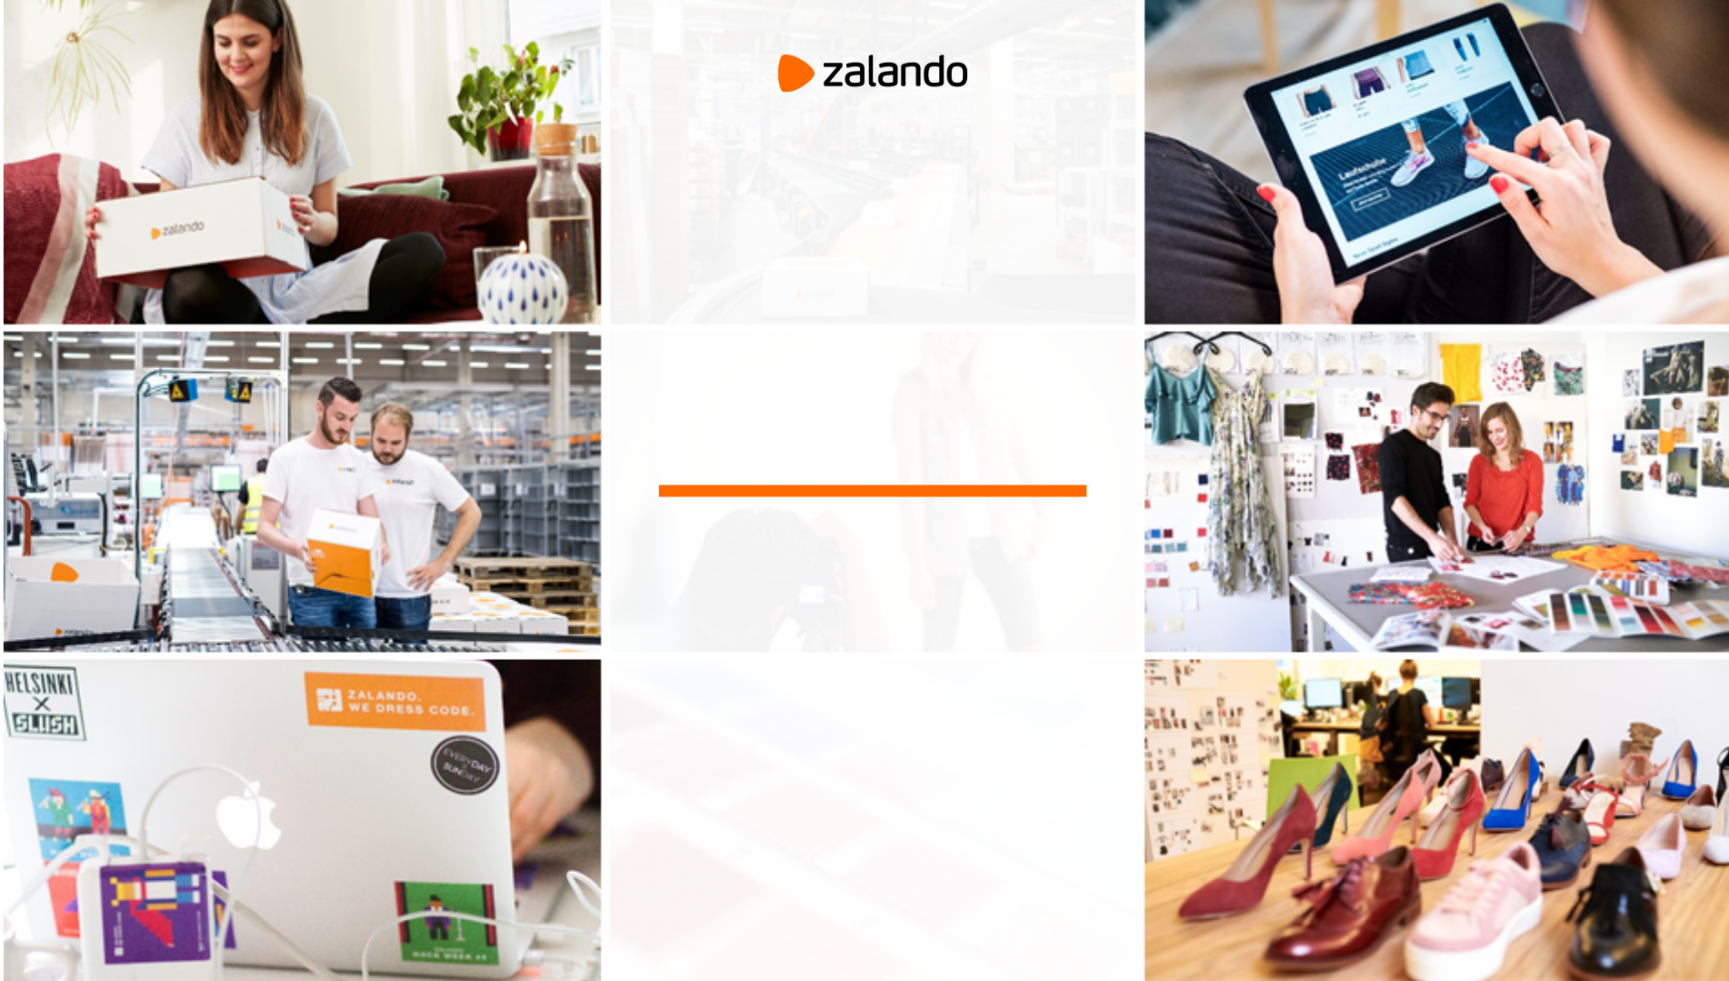
\includegraphics[width=\paperwidth]{template_2.png}}%
  \fontsize{17pt}{18}\selectfont
  \maketitle
}

\AddToShipoutPictureBG{
  \AtPagemyUpperLeft{{
\includegraphics[width=2.0cm,keepaspectratio]{logo.png}}}
}%

\setbeamertemplate{background canvas}{
\begin{tikzpicture}
    \clip (0,0) rectangle (\paperwidth,\paperheight);
    \fill[color=orange] (4cm, \paperheight-6pt) rectangle (\paperwidth-4cm,\paperheight);
\end{tikzpicture}
}

\fontsize{17pt}{18}\selectfont

\begin{frame}
    \frametitle{}
    \begin{minipage}{14cm}
        \begin{center}

        \vspace{10mm}
        
\includegraphics[width=1.0\textwidth,center]{acid_team.png}

        \vspace{5mm}

        \href{https://github.com/zalando/patroni}
             {\color{black}\normalsize{patroni}} \&
        \href{https://github.com/zalando-incubator/postgres-operator}
             {\color{black}\normalsize{postgres-operator}}
        \end{center}
    \end{minipage}
\end{frame}

\begin{frame}[fragile]{}
    \frametitle{}
    \begin{columns}
        \begin{column}{0.48\columnwidth}
        \begin{minted}[fontsize=\normalsize]{yaml}
        resources:
          requests:
            cpu: "1000m"
            memory: "1GB"
          limits:
            cpu: "2000m"
            memory: "2GB"
        \end{minted}
        \end{column}

        \begin{column}{0.48\columnwidth}
            \vspace*{-2.5em}
            \begin{center}
            \fontsize{88pt}{90}\selectfont{\color{black} \textbf{?}}
            \end{center}
        \end{column}

    \end{columns}
\end{frame}

\begin{frame}[fragile]{}
    \frametitle{}
    \begin{center}
        \textbf{Allocatable}

        \begin{onlyenv}<1>
            \begin{minted}[fontsize=\normalsize,escapeinside=??]{bash}
            Capacity:
             cpu:                         16
             hugepages-1Gi:               0
             hugepages-2Mi:               0
             memory:                      65947396Ki
            Allocatable:
             cpu:                         15800m
             hugepages-1Gi:               0
             hugepages-2Mi:               0
             memory:                      65388292Ki
            \end{minted}

            \vspace{-6.0cm}
            \begin{tikzpicture}
                \draw[
                    transparent=1.0,
                    color=red,
                    line width=1.5mm,
                    rotate=10,
                    pattern=north west lines,
                    pattern color=red!30
                ] (0, 0) ellipse (4cm and 2cm) node[pos=0.0] {
                    \fontsize{28pt}{28}\selectfont
                    {\textbf{K8S appliance?}
                    }};
            \end{tikzpicture}
        \end{onlyenv}

        \begin{onlyenv}<2>
            \color{gray}
            \begin{minted}[fontsize=\normalsize,escapeinside=??]{bash}
            Capacity:
             cpu:                         16
             hugepages-1Gi:               0
             hugepages-2Mi:               0
             memory:                      65947396Ki
            Allocatable:
             cpu:                         15800m
             hugepages-1Gi:               0
             hugepages-2Mi:               0
             memory:                      65388292Ki
            \end{minted}

            \vspace{-6.0cm}
            \begin{tikzpicture}
                \draw[
                    color=red,
                    line width=1.5mm,
                    rotate=10,
                    pattern=north west lines,
                    pattern color=red!30
                ] (0, 0) ellipse (4cm and 2cm) node[pos=0.0] {
                    \fontsize{28pt}{28}\selectfont
                    {\textbf{K8S appliance?}
                    }};
            \end{tikzpicture}
        \end{onlyenv}
    \end{center}
\end{frame}

\begin{frame}
    \frametitle{}
    \begin{center}
        \vspace{1.0cm}

        \only<1>{
        \begin{tikzpicture}[component/.style={
                regular polygon,
                regular polygon sides=4,
                rounded corners,
                line width=0.5mm,
        }]
            \draw[component, color=white] (0, 0) rectangle (2.8, 2.8) node[pos=0.5] {\textbf{cgroups}};
            \draw[component, color=white] (3.2, 3.2) rectangle (6.0, 6.0) node[pos=0.5] {\textbf{caps}};
            \draw[component, color=white] (0, 3.2) rectangle (2.8, 6.0) node[pos=0.5] {\textbf{ns}};
            \draw[component, color=white] (3.2, 0) rectangle (6.0, 2.8) node[pos=0.5] {\textbf{root}};
        \end{tikzpicture}
        }

        \only<2>{
        \begin{tikzpicture}[component/.style={
                regular polygon,
                regular polygon sides=4,
                rounded corners,
                line width=0.5mm,
        }]
            \draw[component, fill=blue!20] (0, 0) rectangle (2.8, 2.8) node[pos=0.5] {\textbf{cgroups}};
            \draw[component, color=white] (3.2, 3.2) rectangle (6.0, 6.0) node[pos=0.5] {\textbf{caps}};
            \draw[component, color=white] (0, 3.2) rectangle (2.8, 6.0) node[pos=0.5] {\textbf{ns}};
            \draw[component, color=white] (3.2, 0) rectangle (6.0, 2.8) node[pos=0.5] {\textbf{root}};
        \end{tikzpicture}
        }

        \only<3>{
        \begin{tikzpicture}[component/.style={
                regular polygon,
                regular polygon sides=4,
                rounded corners,
                line width=0.5mm,
        }]
            \draw[component, fill=blue!20] (0, 0) rectangle (2.8, 2.8) node[pos=0.5] {\textbf{cgroups}};
            \draw[component, color=white] (3.2, 3.2) rectangle (6.0, 6.0) node[pos=0.5] {\textbf{caps}};
            \draw[component, fill=red!20] (0, 3.2) rectangle (2.8, 6.0) node[pos=0.5] {\textbf{ns}};
            \draw[component, color=white] (3.2, 0) rectangle (6.0, 2.8) node[pos=0.5] {\textbf{root}};
        \end{tikzpicture}
        }

        \only<4>{
        \begin{tikzpicture}[component/.style={
                regular polygon,
                regular polygon sides=4,
                rounded corners,
                line width=0.5mm,
        }]
            \draw[component, fill=blue!20] (0, 0) rectangle (2.8, 2.8) node[pos=0.5] {\textbf{cgroups}};
            \draw[component, fill=green!20] (3.2, 3.2) rectangle (6.0, 6.0) node[pos=0.5] {\textbf{caps}};
            \draw[component, fill=red!20] (0, 3.2) rectangle (2.8, 6.0) node[pos=0.5] {\textbf{ns}};
            \draw[component, color=white] (3.2, 0) rectangle (6.0, 2.8) node[pos=0.5] {\textbf{root}};
        \end{tikzpicture}
        }

        \only<5>{
        \begin{tikzpicture}[component/.style={
                regular polygon,
                regular polygon sides=4,
                rounded corners,
                line width=0.5mm,
        }]
            \draw[component, fill=blue!20] (0, 0) rectangle (2.8, 2.8) node[pos=0.5] {\textbf{cgroups}};
            \draw[component, fill=green!20] (3.2, 3.2) rectangle (6.0, 6.0) node[pos=0.5] {\textbf{caps}};
            \draw[component, fill=red!20] (0, 3.2) rectangle (2.8, 6.0) node[pos=0.5] {\textbf{ns}};
            \draw[component, fill=yellow!20] (3.2, 0) rectangle (6.0, 2.8) node[pos=0.5] {\textbf{root}};
        \end{tikzpicture}
        }

        \href{https://github.com/opencontainers/runc/blob/master/libcontainer/SPEC.md}
        {\color{black}\normalsize{libcontainer/SPEC.md}}
    \end{center}
\end{frame}
\note{
    root is about chroot/pivot_root
}

\begin{frame}[fragile]{}
    \frametitle{}

    \only<1>{
        \begin{center}
        \begin{tikzpicture}[]

        \def\firstcircle{(0,0) circle (1.5cm)}
        \def\secondcircle{(60:4cm) circle (1.5cm)}
        \def\thirdcircle{(0:4cm) circle (1.5cm)}

        \begin{scope}[shift={(3cm,-5cm)}, fill opacity=0.5, line width=0.5mm]
            \fill[red] \firstcircle;
            \fill[green] \secondcircle;
            \fill[blue] \thirdcircle;

            \draw \firstcircle node [] {\textbf{res}};
            \draw \secondcircle node [] {\textbf{limit}};
            \draw \thirdcircle node [] {\textbf{time}};
        \end{scope}
        \end{tikzpicture}
        \end{center}
    }

    \only<2> {
        \begin{center}
        \begin{tikzpicture}[]

        \def\firstcircle{(0,0) circle (1.5cm)}
        \def\secondcircle{(60:2cm) circle (1.5cm)}
        \def\thirdcircle{(0:2cm) circle (1.5cm)}

        \begin{scope}[shift={(3cm,-5cm)}, fill opacity=0.5, line width=0.5mm]
            \fill[red] \firstcircle;
            \fill[green] \secondcircle;
            \fill[blue] \thirdcircle;

            \draw \firstcircle node [below] {\textbf{res}};
            \draw \secondcircle node [above] {\textbf{limit}};
            \draw \thirdcircle node [below] {\textbf{time}};
        \end{scope}
        \end{tikzpicture}
        \end{center}
    }

\end{frame}

\begin{frame}
    \frametitle{}
    \begin{columns}

        \begin{column}{0.15\columnwidth}
        \end{column}

        \begin{column}{0.35\columnwidth}
        \begin{itemize}[label={\MVRightarrow}]
            \item docker
            \item rkt
            \item LXC
            \item $\cdots$
        \end{itemize}
        \end{column}

        \begin{column}{0.48\columnwidth}
        \begin{itemize}[label={\MVRightarrow}]
            \item podman
            \item cgroup v1
            \item cgroup v2
            \item $\cdots$
        \end{itemize}
        \end{column}

    \end{columns}

\end{frame}

\begin{frame}
    \frametitle{}
    \begin{center}

    \begin{tikzpicture}[
        scale=0.6,
        every node/.style={draw=black!70,fill=red!30,rounded corners,thick,anchor=west, minimum width=4cm,transform shape, blur shadow={shadow blur steps=5,shadow blur extra rounding=1.3pt}, inner sep=.5cm},
        inactive/.style={fill=gray!30},
        to/.style={->,>=stealth',shorten >=1pt,semithick,font=\sffamily\footnotesize},
        ]
      \node [fill=yellow!20] (cgroup-v1) {cgroup v1};
      \node [below=.5cm of cgroup-v1] (cpu) {CPU};
      \node [inactive, left=.5cm of cpu] (systemd) {Systemd};
      \node [inactive, right=.5cm of cpu] (memory) {Memory};
      \node [inactive, right=.5cm of memory, minimum width=1cm, inner sep=0.7cm] (rest) {\ldots};
      \node [below=.5cm of cpu] (k8s) {K8S};
      \node [below=.5cm of k8s] (guaranteed) {Guaranteed};
      \node [inactive, right=.5cm of guaranteed] (burstable) {Burstable};
      \node [inactive, left=.5cm of guaranteed] (bestefforts) {Best Efforts};
      \node [below=.5cm of guaranteed] (pause) {Pause};
      \node [below=.5cm of pause] (app) {App};

      \draw[to] (cgroup-v1) -- (cpu);
      \draw[to] (cgroup-v1) -| (memory);
      \draw[to] (cgroup-v1) -| (rest);
      \draw[to] (cgroup-v1) -| (systemd);
      \draw[to] (cpu) -- (k8s);
      \draw[to] (k8s) -- (guaranteed);
      \draw[to] (k8s) -| (bestefforts);
      \draw[to] (k8s) -| (burstable);
      \draw[to] (guaranteed) -- (pause);
      \draw[to] (pause) -- (app);
    \end{tikzpicture}

    \end{center}
\end{frame}

\begin{frame}[fragile]{}
    \frametitle{}
    \begin{center}

    \begin{columns}
    \begin{column}{0.48\columnwidth}
        \begin{minted}[fontsize=\normalsize,escapeinside=??]{yaml}
        resources:
          requests:
            cpu: "1000m" ?\tikzmark{cpu_req}?
            memory: "1GB"
          limits:
            cpu: "2000m" ?\tikzmark{cpu_lim}?
            memory: "2GB"
        \end{minted}
    \end{column}

    \begin{column}{0.48\columnwidth}
        \begin{tikzpicture}[remember picture,
            every node/.style={
                fill=red!30,
                rounded corners=0.2cm,
                minimum width=3cm,
                inner sep=0.5cm,
            },
            baseline=(cpu_req.south), anchor=base
            ]
          \draw node[] (cpu_shares) {\textbf{cpu share}};
          \draw node[below=0.3 of cpu_shares] (cpu_cfs) {\textbf{cfs quota}};

          \draw [overlay, ->, line width=3pt, red] (cpu_req) -- (cpu_shares.west);
          \draw [overlay, ->, line width=3pt, red] (cpu_lim) -- (cpu_cfs.west);
        \end{tikzpicture}
    \end{column}
    \end{columns}

\end{center}
\end{frame}

\begin{frame}
    \frametitle{}
    \begin{center}
    \textbf{Share}

        \vspace{1.0cm}
        \only<1>{
            \begin{tikzpicture}
                \draw[
                    line width=0.5mm,
                    fill=red!30
                ] (0.0,0.0) rectangle (4.0,2.0) node[pos=.5] {\textbf{C1}};

                \draw[
                    line width=0.5mm,
                    fill=blue!30
                ] (4.0,0.0) rectangle (8.0,2.0) node[pos=.5] {\textbf{C2}};

            \end{tikzpicture}
        }

        \only<2>{
            \begin{tikzpicture}

                \draw[
                    line width=0.5mm,
                    fill=red!30
                ] (0.0,0.0) rectangle (2.0,2.0) node[pos=.5] {\textbf{C1}};

                \draw[
                    line width=0.5mm,
                    fill=blue!30
                ] (2.0,0.0) rectangle (4.0,2.0) node[pos=.5] {\textbf{C2}};

                \draw[
                    line width=0.5mm,
                    fill=green!30
                ] (4.0,0.0) rectangle (6.0,2.0) node[pos=.5] {\textbf{C3}};

                \draw[
                    line width=0.5mm,
                    fill=gray!30
                ] (6.0,0.0) rectangle (8.0,2.0) node[pos=.5] {\textbf{C4}};

            \end{tikzpicture}
        }

    \end{center}
\end{frame}

\begin{frame}
    \frametitle{}
    \begin{center}
    \textbf{Quota}

        \vspace{1.0cm}
        \only<1>{
            \begin{tikzpicture}
                \draw[
                    line width=0.5mm,
                    fill=red!30
                ] (0.0,0.0) rectangle (2.0,2.0) node[pos=.5] {\textbf{C1}};

                \draw[
                    line width=0.5mm,
                    fill=blue!30
                ] (2.0,0.0) rectangle (4.0,2.0) node[pos=.5] {\textbf{C2}};

                \draw[
                    line width=0.5mm,
                    dashed
                ] (4.0,0.0) rectangle (8.0,2.0) node[pos=.5] {};

            \end{tikzpicture}
        }

        \only<2>{
            \begin{tikzpicture}

                \draw[
                    line width=0.5mm,
                    fill=red!30
                ] (0.0,0.0) rectangle (2.0,2.0) node[pos=.5] {\textbf{C1}};

                \draw[
                    line width=0.5mm,
                    fill=blue!30
                ] (2.0,0.0) rectangle (4.0,2.0) node[pos=.5] {\textbf{C2}};

                \draw[
                    line width=0.5mm,
                    fill=green!30
                ] (4.0,0.0) rectangle (6.0,2.0) node[pos=.5] {\textbf{C3}};

                \draw[
                    line width=0.5mm,
                    fill=gray!30
                ] (6.0,0.0) rectangle (8.0,2.0) node[pos=.5] {\textbf{C4}};

            \end{tikzpicture}
        }

    \end{center}
\end{frame}

\begin{frame}[fragile]{}
    \frametitle{}
    \begin{center}
        \textbf{Bandwidth accounting}

        \begin{flushleft}
        \begin{minted}[fontsize=\LARGE]{bash}
# from /proc/sys/kernel/
sched_cfs_bandwidth_slice_us
# default=5ms
        \end{minted}
        \end{flushleft}

    \end{center}
\end{frame}

\begin{frame}[fragile]{}
    \frametitle{}
    \begin{center}
        \textbf{Exclusive CPU}

        \begin{itemize}[label={\MVRightarrow}]
            \item cpu management policy
            \item kube-reserved
			\item guaranteed (integer quantity)
            \item cpuset.cpus
            \item cpuset.cpuset.cpu\_exclusive
        \end{itemize}

    \end{center}
\end{frame}

\begin{frame}[fragile]{}
    \frametitle{}
    \begin{center}

    \begin{overprint}
    \onslide<1>
        \begin{columns}
        \begin{column}{0.48\columnwidth}
            \begin{minted}[fontsize=\normalsize,escapeinside=??]{yaml}
            resources:
              requests:
                cpu: "1000m"
                memory: "1GB" ?\tikzmark{mem_req}?
              limits:
                cpu: "2000m"
                memory: "2GB" ?\tikzmark{mem_lim}?
            \end{minted}
        \end{column}

        \begin{column}{0.48\columnwidth}
            \begin{tikzpicture}[remember picture,
                every node/.style={
                    fill=red!30,
                    rounded corners=0.2cm,
                    minimum width=3cm,
                    inner sep=0.5cm,
                },
                baseline=(mem_req.south), anchor=base
                ]
              \draw node[] (soft_mem) {\textbf{soft mem limit}};
              \draw node[below=0.3 of soft_mem] (hard_mem) {\textbf{hard mem limit}};

              \draw [overlay, ->, line width=3pt, red] (mem_req) -- (soft_mem.west);
              \draw [overlay, ->, line width=3pt, red] (mem_lim) -- (hard_mem.west);

              \draw[
                  -,
                  line width=1.75mm,
                  color=red,
                  transparent=1.0,
              ] (soft_mem.south west) to (soft_mem.north east);

              \draw[
                  -,
                  line width=1.75mm,
                  color=red,
                  transparent=1.0,
              ] (soft_mem.south east) to (soft_mem.north west);

            \end{tikzpicture}
        \end{column}
        \end{columns}

    \onslide<2>
        \begin{columns}
        \begin{column}{0.48\columnwidth}
            \begin{minted}[fontsize=\normalsize,escapeinside=??]{yaml}
            resources:
              requests:
                cpu: "1000m"
                memory: "1GB" ?\tikzmark{mem_req}?
              limits:
                cpu: "2000m"
                memory: "2GB" ?\tikzmark{mem_lim}?
            \end{minted}
        \end{column}

        \begin{column}{0.48\columnwidth}
            \begin{tikzpicture}[remember picture,
                every node/.style={
                    fill=red!30,
                    rounded corners=0.2cm,
                    minimum width=3cm,
                    inner sep=0.5cm,
                },
                baseline=(mem_req.south), anchor=base
                ]
              \draw node[] (soft_mem) {\textbf{soft mem limit}};
              \draw node[below=0.3 of soft_mem] (hard_mem) {\textbf{hard mem limit}};

              \draw [overlay, ->, line width=3pt, red, transparent=1.0] (mem_req) -- (soft_mem.west);
              \draw [overlay, ->, line width=3pt, red] (mem_lim) -- (hard_mem.west);

              \draw[
                  -,
                  line width=1.75mm,
                  color=red,
              ] (soft_mem.south west) to (soft_mem.north east);

              \draw[
                  -,
                  line width=1.75mm,
                  color=red,
              ] (soft_mem.south east) to (soft_mem.north west);
            \end{tikzpicture}
        \end{column}
        \end{columns}
\end{overprint}

\end{center}
\end{frame}

\begin{frame}[fragile]{}
    \frametitle{}
    \begin{center}
        \textbf{Memory reclaim}

        \begin{flushleft}
        \begin{minted}[fontsize=\normalsize]{bash}
# only under the memory pressure
=> page_reclaim.py --container 89c33bb3133f

[7382] postgres: 928K
[7138] postgres: 152K
[7136] postgres: 180K
[7468] postgres: 72M
[7464] postgres: 57M
[5451] postgres: 1M
        \end{minted}
        \end{flushleft}

    \end{center}
\end{frame}

\begin{frame}
    \frametitle{}
    \begin{center}
    \textbf{Memory}

        \begin{itemize}[label={\MVRightarrow}]
            \item best efforts
            \item requests for QoS and oom\_adj
            \item memory.kmem.limit\_in\_bytes
            \item MEMCG\_CHARGE\_BATCH (32 pages)
            \item shared memory CoW
        \end{itemize}

    \end{center}
\end{frame}
\note{
    kmem limit attributed as part of mem limit
}

\begin{frame}[fragile]{}
    \frametitle{}
    \begin{columns}
        \begin{column}{0.48\columnwidth}
        \begin{minted}[fontsize=\normalsize]{yaml}
    resources:
      requests:
        cpu: "1000m"
        memory: "1GB"
        hugepages-1Gi: "1GB"
        hugepages-2Mi: "1GB"
      limits:
        cpu: "2000m"
        memory: "2GB"
        hugepages-1Gi: "2GB"
        hugepages-2Mi: "2GB"
        \end{minted}
        \end{column}

        \begin{column}{0.48\columnwidth}
            \vspace*{-2.5em}
            \begin{center}
                \begin{itemize}
                    \item <+->
                \end{itemize}

                \begin{itemize}[label={\MVRightarrow}]
                    \item classic
                    \item \sout{transparent}
                    \item isolation only per pod
                    \item no soft limits or reclaim (SIGBUS)
                \end{itemize}
            \end{center}
        \end{column}

    \end{columns}
\end{frame}

\begin{frame}[fragile]{}
    \frametitle{}
    \begin{center}
        \textbf{Huge pages experiment}

    \begin{overprint}
        \onslide<1>
        \begin{flushleft}
        \begin{minted}[fontsize=\normalsize,escapeinside=||]{python}
# perf record -e dTLB-loads,dTLB-stores -p PID
# huge_pages on
Samples: 832K of event 'dTLB-load-misses'
Event count (approx.): 640614445 : |\colorbox{White}{\textbf{~19%}}| less
Samples: 736K of event 'dTLB-store-misses'
Event count (approx.): 72447300 : |\colorbox{White}{\textbf{~29%}}| less

# huge_pages off
Samples: 894K of event 'dTLB-load-misses'
Event count (approx.): 784439650
Samples: 822K of event 'dTLB-store-misses'
Event count (approx.): 101471557
        \end{minted}
        \end{flushleft}

        \onslide<2>
        \begin{flushleft}
        \begin{minted}[fontsize=\normalsize,escapeinside=||]{python}
# perf record -e dTLB-loads,dTLB-stores -p PID
# huge_pages on
Samples: 832K of event 'dTLB-load-misses'
Event count (approx.): 640614445 : |\colorbox{RedOrange}{\textbf{~19%}}| less
Samples: 736K of event 'dTLB-store-misses'
Event count (approx.): 72447300 : |\colorbox{RedOrange}{\textbf{~29%}}| less

# huge_pages off
Samples: 894K of event 'dTLB-load-misses'
Event count (approx.): 784439650
Samples: 822K of event 'dTLB-store-misses'
Event count (approx.): 101471557
        \end{minted}
        \end{flushleft}

    \end{overprint}
    \end{center}
\end{frame}

\begin{frame}[fragile]{}
    \frametitle{}
    \begin{columns}
        \begin{column}{0.48\columnwidth}
        \begin{minted}[fontsize=\normalsize]{yaml}

    resources:
      requests:
        cpu: "1000m"
        memory: "1GB"
        hugepages-1Gi: "1GB"
        hugepages-2Mi: "1GB"
      limits:
        cpu: "2000m"
        memory: "2GB"
        hugepages-1Gi: "2GB"
        hugepages-2Mi: "2GB"
        \end{minted}
        \end{column}

        \begin{column}{0.48\columnwidth}
            \vspace*{-2.5em}
            \begin{center}
            \fontsize{28pt}{30}\selectfont{\color{black} \textbf{What is missing?}}
            \end{center}
        \end{column}

    \end{columns}
\end{frame}

\begin{frame}[fragile]{}
    \frametitle{}
    \begin{columns}
        \begin{column}{0.48\columnwidth}
        \begin{minted}[fontsize=\normalsize]{yaml}

    resources:
      requests:
        cpu: "1000m"
        memory: "1GB"
        hugepages-1Gi: "1GB"
        hugepages-2Mi: "1GB"
      limits:
        cpu: "2000m"
        memory: "2GB"
        hugepages-1Gi: "2GB"
        hugepages-2Mi: "2GB"
        \end{minted}
        \end{column}

        \begin{column}{0.48\columnwidth}
            \begin{center}
            \begin{minted}[fontsize=\normalsize]{yaml}
resources:
  requests:
    io: "?"
    llcache: "?"
    network: "?"

  limits:
    io: "?"
    llcache: "?"
    network: "?"

            \end{minted}
            \end{center}
        \end{column}

    \end{columns}
\end{frame}

%\begin{frame}[fragile]{}
    %\frametitle{}
    %\begin{center}
        %\textbf{LLCache}

        %\begin{flushleft}
		%\begin{minted}[fontsize=\normalsize]{bash}
%=> pqos -s
%L3CA COS definitions for Socket 0:
	%L3CA COS0 => MASK 0xffff
	%L3CA COS1 => MASK 0xf
	%L3CA COS2 => MASK 0xff0
	%L3CA COS3 => MASK 0xfff
%Core information for socket 0:
	%Core 0, L2ID 0, L3ID 0 => COS0
	%Core 1, L2ID 1, L3ID 0 => COS0
	%Core 2, L2ID 0, L3ID 0 => COS0
	%Core 3, L2ID 1, L3ID 0 => COS0
        %\end{minted}
        %\end{flushleft}

    %\end{center}
%\end{frame}

%\begin{frame}[fragile]{}
    %\frametitle{}
    %\begin{center}
        %\textbf{LLCache}

        %\begin{flushleft}
		%\begin{minted}[fontsize=\normalsize]{bash}
%# COS1 4 cache ways, COS 2 next 8 cache ways
%=> pqos -e "llc:1=0x000f;llc:2=0x0ff0;"
%SOCKET 0 L3CA COS1 => MASK 0xf
%SOCKET 0 L3CA COS2 => MASK 0xff0
%Allocation configuration altered.
        %\end{minted}
        %\end{flushleft}

    %\end{center}
%\end{frame}

\begin{frame}
    \frametitle{}
    \begin{center}
    \textbf{Block I/O}

            \begin{itemize}
                \item <+->
            \end{itemize}

            \begin{itemize}[label={\MVRightarrow}]
                \item<+-> sharing a disk between users in Linux is awful
                \item<+-> throttling puts pressure somewhere else
                \item<+-> lack of trivially observable cost metric
            \end{itemize}

        \normalsize{\href{https://lwn.net/Articles/782876/}
                   {\color{black}The creation of the io.latency block I/O controller}}

    \end{center}
\end{frame}

\begin{frame}[fragile]{}
    \frametitle{}
    \begin{center}
        \textbf{Writeback monitoring}

        \begin{flushleft}
        \begin{minted}[fontsize=\normalsize]{bash}
=> perf record -e writeback:writeback_written

kworker/u8:1 reason=periodic   nr_pages=101429
kworker/u8:1 reason=background nr_pages=MAX_ULONG
kworker/u8:3 reason=periodic   nr_pages=101457
        \end{minted}
        \end{flushleft}

    \end{center}
\end{frame}

\begin{frame}[fragile]{}
    \frametitle{}
    \begin{center}
        \textbf{Writeback monitoring}

        \begin{flushleft}
        \begin{minted}[fontsize=\normalsize]{bash}
# pgbench insert workload
=> io_timeouts.py bin/postgres

[18335] END: MAX_SCHEDULE_TIMEOUT
[18333] END: MAX_SCHEDULE_TIMEOUT
[18331] END: MAX_SCHEDULE_TIMEOUT
[18318] truncate pgbench_history: MAX_SCHEDULE_TIMEOUT
        \end{minted}
        \end{flushleft}

    \end{center}
\end{frame}

\begin{frame}
    \frametitle{}
    \begin{center}
    \textbf{blkio cgroup v1}

        \begin{itemize}[label={\MVRightarrow}]
            \item Direct IO oriented
            \item no relationships between controllers
            \item writeback = memory + blkio controllers
            \item writeback accounted to the root cgroup
        \end{itemize}

        \normalsize{\href{
            https://git.kernel.org/pub/scm/linux/kernel/git/torvalds/linux.git/commit/?h=v4.14-rc4&id=3e1534cf4a2a8278e811e7c84a79da1a02347b8b
        }{\color{black}https://git.kernel.org/pub/scm/linux/kernel/git/torvalds/linux.git}}

    \end{center}
\end{frame}

\begin{frame}[fragile]{}
    \frametitle{}
    \begin{center}
        \textbf{IO scheduler}

        \begin{flushleft}
		\begin{minted}[fontsize=\LARGE]{bash}
=> cat /sys/block/xvdcj/queue/scheduler
[mq-deadline] kyber bfq none
        \end{minted}
        \end{flushleft}

    \end{center}
\end{frame}

\begin{frame}[fragile]{}
    \frametitle{}
    \begin{center}
        \begin{overprint}

        \onslide<1>
        \begin{tikzpicture}[
            queue/.style={line width=0.5mm},
            connection/.style={-,>=stealth',semithick,rounded corners=5pt}
            ]
            \draw[fill=gray!20, rounded corners] (0, 0) rectangle (12, 8) node[pos=0.5] {};
            \draw[fill=gray!40, rounded corners] (0.2, 0.2) rectangle (5.8, 7.8) node[pos=0.5, text depth=6cm] {I/O sched};
            \draw[fill=gray!40, text depth=6cm] (6.2, 0.2) rectangle (11.8, 7.8) node[pos=0.5] {blkmq};

            \draw[fill=yellow!60, rounded corners] (0.4, 5.3) rectangle (2.2, 6.0) node[pos=0.5] (noop) {\normalsize{\textbf{noop}}};
            \coordinate[above=0.5 of noop] (noop-arrow);
            \draw[fill=yellow!60, rounded corners] (1.9, 4.4) rectangle (3.7, 5.1) node[pos=0.5] (cfq) {\normalsize{\textbf{cfq}}};
            \coordinate[above=0.5 of cfq] (cfq-arrow);
            \draw[fill=yellow!60, rounded corners] (3.4, 3.5) rectangle (5.2, 4.2) node[pos=0.5] (deadline) {\normalsize{\textbf{deadline}}};
            \coordinate[above=0.5 of deadline] (deadline-arrow);

            \draw[connection, ->] (noop-arrow) to (noop);
            \draw[connection, ->] (cfq-arrow) to (cfq);
            \draw[connection, ->] (deadline-arrow) to (deadline);

            \draw [thick,decorate,decoration={brace,amplitude=5pt}]
                (2.75, 2.0)  -- (2.75, 0.4)
                node[black, midway, right=4pt, font=\normalsize, text width=3cm] {Hardware\\queue};

            \draw[fill=yellow!60, rounded corners] (0.4 + 6, 5.3) rectangle (2.2 + 6, 6.0) node[pos=0.5] (none) {\normalsize{\textbf{none}}};
            \coordinate[above=0.5 of none] (none-arrow);
            \draw[fill=yellow!60, rounded corners] (2.4 + 6, 5.3) rectangle (4.4 + 6, 6.0) node[pos=0.5] (kyber) {\normalsize{\textbf{kyber}}};
            \coordinate[above=0.5 of kyber] (kyber-arrow);
            \draw[fill=yellow!60, rounded corners] (4.6 + 6, 5.3) rectangle (5.4 + 6, 6.0) node[pos=0.5] (others)  {\normalsize{\textbf{...}}};
            \coordinate[above=0.5 of others] (others-arrow);

            \draw[connection, ->, shorten >=2pt] (none-arrow) to (none);
            \draw[connection, ->] (kyber-arrow) to (kyber.north);
            \draw[connection, ->, shorten >=3pt] (others-arrow) to (others.north);

            \draw[queue] (2.0, 0.4) rectangle (2.5, 0.8) node[pos=0.5] {};
            \draw[queue] (2.0, 0.8) rectangle (2.5, 1.2) node[pos=0.5] {};
            \draw[queue] (2.0, 1.2) rectangle (2.5, 1.6) node[pos=0.5] {};
            \draw[queue] (2.0, 1.6) rectangle (2.5, 2.0) node[pos=0.5] (top-hw-sched) {};
            \coordinate[above=0.5 of top-hw-sched] (hw-sched-arrow);
            \draw[connection, ->] (hw-sched-arrow) to (top-hw-sched.north);
            \draw[connection] (noop.south) |- (hw-sched-arrow);
            \draw[connection, rounded corners=0pt] (cfq.south) |- (hw-sched-arrow);
            \draw[connection] (deadline.south) |- (hw-sched-arrow);

            \draw[queue] (7.0 + 0.5, 0.4) rectangle (7.5 + 0.5, 0.8) node[pos=0.5] {};
            \draw[queue] (7.0 + 0.5, 0.8) rectangle (7.5 + 0.5, 1.2) node[pos=0.5] {};
            \draw[queue] (7.0 + 0.5, 1.2) rectangle (7.5 + 0.5, 1.6) node[pos=0.5] {};
            \draw[queue] (7.0 + 0.5, 1.6) rectangle (7.5 + 0.5, 2.0) node[pos=0.5] (hw-queue-2) {};

            \draw[queue] (9.0 - 0.5, 0.4) rectangle (9.5 - 0.5, 0.8) node[pos=0.5] {};
            \draw[queue] (9.0 - 0.5, 0.8) rectangle (9.5 - 0.5, 1.2) node[pos=0.5] {};
            \draw[queue] (9.0 - 0.5, 1.2) rectangle (9.5 - 0.5, 1.6) node[pos=0.5] {};
            \draw[queue] (9.0 - 0.5, 1.6) rectangle (9.5 - 0.5, 2.0) node[pos=0.5] (hw-queue-1) {};

            \draw [thick,decorate,decoration={brace,amplitude=5pt}]
                (9.25, 2.0)  -- (9.25, 0.4)
                node[black, midway, right=4pt, font=\normalsize, text width=3cm] {Hardware\\queue};

            \draw[queue] (7.0, 0.4 + 2.5) rectangle (7.5, 0.8 + 2.5) node[pos=0.5] (sw-3-bottom) {};
            \draw[queue] (7.0, 0.8 + 2.5) rectangle (7.5, 1.2 + 2.5) node[pos=0.5] {};
            \draw[queue] (7.0, 1.2 + 2.5) rectangle (7.5, 1.6 + 2.5) node[pos=0.5] {};
            \draw[queue] (7.0, 1.6 + 2.5) rectangle (7.5, 2.0 + 2.5) node[pos=0.5] (sw-3) {};
            \coordinate[above=0.25 of sw-3] (sw-3-low);

            \draw[queue] (8.0, 0.4 + 2.5) rectangle (8.5, 0.8 + 2.5) node[pos=0.5] (sw-2-bottom) {};
            \draw[queue] (8.0, 0.8 + 2.5) rectangle (8.5, 1.2 + 2.5) node[pos=0.5] {};
            \draw[queue] (8.0, 1.2 + 2.5) rectangle (8.5, 1.6 + 2.5) node[pos=0.5] {};
            \draw[queue] (8.0, 1.6 + 2.5) rectangle (8.5, 2.0 + 2.5) node[pos=0.5] (sw-2) {};
            \coordinate[above=0.25 of sw-2] (sw-2-low);
            \coordinate[below=0.5 of sw-2-bottom] (sw-2-connection);

            \draw[queue] (9.0, 0.4 + 2.5) rectangle (9.5, 0.8 + 2.5) node[pos=0.5] (top-sw-bottom) {};
            \draw[queue] (9.0, 0.8 + 2.5) rectangle (9.5, 1.2 + 2.5) node[pos=0.5] {};
            \draw[queue] (9.0, 1.2 + 2.5) rectangle (9.5, 1.6 + 2.5) node[pos=0.5] {};
            \draw[queue] (9.0, 1.6 + 2.5) rectangle (9.5, 2.0 + 2.5) node[pos=0.5] (top-sw-queue) {};
            \coordinate[above=0.5 of top-sw-queue] (sw-queue-arrow);
            \draw[connection] (none.south) |- (sw-queue-arrow.north);
            \draw[connection, rounded corners=0pt] (kyber.south) |- (sw-queue-arrow.north);
            \draw[connection] (others.south) |- (sw-queue-arrow.north);

            \coordinate[above=0.25 of top-sw-queue] (sw-queue-arrow-low);
            \draw[connection, rounded corners=0pt] (sw-queue-arrow-low) |- (top-sw-queue.north);
            \draw[connection, rounded corners=0pt] (sw-queue-arrow-low) |- (sw-2-low.north);
            \draw[connection, rounded corners=0pt] (sw-queue-arrow-low) |- (sw-3-low.north);

            \draw[connection, rounded corners=0pt] (sw-queue-arrow-low) -- (sw-queue-arrow);
            \draw[connection, rounded corners=0pt] (sw-2-low) -- (sw-2);
            \draw[connection, rounded corners=0pt] (sw-3-low) -- (sw-3);

            \draw[connection, rounded corners=0pt] (sw-3-low) -- (sw-3);

            \draw[connection, rounded corners=0pt] (sw-2-connection) -| (hw-queue-1.north);
            \draw[connection, rounded corners=0pt] (sw-2-connection) -| (hw-queue-2.north);

            \draw[connection, rounded corners=0pt] (sw-3-bottom) |- (sw-2-connection);
            \draw[connection, rounded corners=0pt] (sw-2-bottom) |- (sw-2-connection);
            \draw[connection, rounded corners=0pt] (top-sw-bottom) |- (sw-2-connection);

            \draw [thick,decorate,decoration={brace,amplitude=5pt}]
                (9.75, 2.0 + 2.5)  -- (9.75, 0.4 + 2.5)
                node[black, midway, right=4pt, font=\normalsize, text width=3cm] {Software\\queue};
        \end{tikzpicture}

        \onslide<2>
        \begin{tikzpicture}[
            queue/.style={line width=0.5mm},
            connection/.style={-,>=stealth',semithick,rounded corners=5pt}
            ]
            \draw[fill=gray!20, rounded corners] (0, 0) rectangle (12, 8) node[pos=0.5] {};
            \draw[fill=gray!40, rounded corners] (0.2, 0.2) rectangle (5.8, 7.8) node[pos=0.5, text depth=6cm] {I/O sched};
            \draw[fill=gray!40, text depth=6cm] (6.2, 0.2) rectangle (11.8, 7.8) node[pos=0.5] {blkmq};

            \draw[fill=yellow!60, rounded corners] (0.4, 5.3) rectangle (2.2, 6.0) node[pos=0.5] (noop) {\normalsize{\textbf{noop}}};
            \coordinate[above=0.5 of noop] (noop-arrow);
            \draw[fill=yellow!60, rounded corners] (1.9, 4.4) rectangle (3.7, 5.1) node[pos=0.5] (cfq) {\normalsize{\textbf{cfq}}};
            \coordinate[above=0.5 of cfq] (cfq-arrow);
            \draw[fill=yellow!60, rounded corners] (3.4, 3.5) rectangle (5.2, 4.2) node[pos=0.5] (deadline) {\normalsize{\textbf{deadline}}};
            \coordinate[above=0.5 of deadline] (deadline-arrow);

            \draw[connection, ->] (noop-arrow) to (noop);
            \draw[connection, ->] (cfq-arrow) to (cfq);
            \draw[connection, ->] (deadline-arrow) to (deadline);

            \draw [thick,decorate,decoration={brace,amplitude=5pt}]
                (2.75, 2.0)  -- (2.75, 0.4)
                node[black, midway, right=4pt, font=\normalsize, text width=3cm] {Hardware\\queue};

            \draw[fill=yellow!60, rounded corners] (0.4 + 6, 5.3) rectangle (2.2 + 6, 6.0) node[pos=0.5] (none) {\normalsize{\textbf{none}}};
            \coordinate[above=0.5 of none] (none-arrow);
            \draw[
                fill=red!20,
                dashed,
                rounded corners,
                line width=0.2mm
            ]
            (2.4 + 6 - 0.1, 5.3 - 0.1) rectangle (4.4 + 6 + 0.1, 6.0 + 0.1)
            node[pos=0.5] {};
            \draw[fill=yellow!60, rounded corners] (2.4 + 6, 5.3) rectangle (4.4 + 6, 6.0) node[pos=0.5] (kyber) {\normalsize{\textbf{kyber}}};
            \coordinate[above=0.5 of kyber] (kyber-arrow);
            \draw[fill=yellow!60, rounded corners] (4.6 + 6, 5.3) rectangle (5.4 + 6, 6.0) node[pos=0.5] (others)  {\normalsize{\textbf{...}}};
            \coordinate[above=0.5 of others] (others-arrow);

            \draw[connection, ->, shorten >=2pt] (none-arrow) to (none);
            \draw[connection, ->] (kyber-arrow) to (kyber.north);
            \draw[connection, ->, shorten >=3pt] (others-arrow) to (others.north);

            \draw[queue] (2.0, 0.4) rectangle (2.5, 0.8) node[pos=0.5] {};
            \draw[queue] (2.0, 0.8) rectangle (2.5, 1.2) node[pos=0.5] {};
            \draw[queue] (2.0, 1.2) rectangle (2.5, 1.6) node[pos=0.5] {};
            \draw[queue] (2.0, 1.6) rectangle (2.5, 2.0) node[pos=0.5] (top-hw-sched) {};
            \coordinate[above=0.5 of top-hw-sched] (hw-sched-arrow);
            \draw[connection, ->] (hw-sched-arrow) to (top-hw-sched.north);
            \draw[connection] (noop.south) |- (hw-sched-arrow);
            \draw[connection, rounded corners=0pt] (cfq.south) |- (hw-sched-arrow);
            \draw[connection] (deadline.south) |- (hw-sched-arrow);

            \draw[queue] (7.0 + 0.5, 0.4) rectangle (7.5 + 0.5, 0.8) node[pos=0.5] {};
            \draw[queue] (7.0 + 0.5, 0.8) rectangle (7.5 + 0.5, 1.2) node[pos=0.5] {};
            \draw[queue] (7.0 + 0.5, 1.2) rectangle (7.5 + 0.5, 1.6) node[pos=0.5] {};
            \draw[queue] (7.0 + 0.5, 1.6) rectangle (7.5 + 0.5, 2.0) node[pos=0.5] (hw-queue-2) {};

            \draw[queue, fill=black!50] (9.0 - 0.5, 0.4) rectangle (9.5 - 0.5, 0.8) node[pos=0.5] {};
            \draw[queue, fill=black!50] (9.0 - 0.5, 0.8) rectangle (9.5 - 0.5, 1.2) node[pos=0.5] {};
            \draw[queue] (9.0 - 0.5, 1.2) rectangle (9.5 - 0.5, 1.6) node[pos=0.5] {};
            \draw[queue] (9.0 - 0.5, 1.6) rectangle (9.5 - 0.5, 2.0) node[pos=0.5] (hw-queue-1) {};

            \draw [thick,decorate,decoration={brace,amplitude=5pt}]
                (9.25, 2.0)  -- (9.25, 0.4)
                node[black, midway, right=4pt, font=\normalsize, text width=3cm] {Hardware\\queue};

            \draw[queue] (7.0, 0.4 + 2.5) rectangle (7.5, 0.8 + 2.5) node[pos=0.5] (sw-3-bottom) {};
            \draw[queue] (7.0, 0.8 + 2.5) rectangle (7.5, 1.2 + 2.5) node[pos=0.5] {};
            \draw[queue] (7.0, 1.2 + 2.5) rectangle (7.5, 1.6 + 2.5) node[pos=0.5] {};
            \draw[queue] (7.0, 1.6 + 2.5) rectangle (7.5, 2.0 + 2.5) node[pos=0.5] (sw-3) {};
            \coordinate[above=0.25 of sw-3] (sw-3-low);

            \draw[queue] (8.0, 0.4 + 2.5) rectangle (8.5, 0.8 + 2.5) node[pos=0.5] (sw-2-bottom) {};
            \draw[queue] (8.0, 0.8 + 2.5) rectangle (8.5, 1.2 + 2.5) node[pos=0.5] {};
            \draw[queue] (8.0, 1.2 + 2.5) rectangle (8.5, 1.6 + 2.5) node[pos=0.5] {};
            \draw[queue] (8.0, 1.6 + 2.5) rectangle (8.5, 2.0 + 2.5) node[pos=0.5] (sw-2) {};
            \coordinate[above=0.25 of sw-2] (sw-2-low);
            \coordinate[below=0.5 of sw-2-bottom] (sw-2-connection);

            \draw[queue] (9.0, 0.4 + 2.5) rectangle (9.5, 0.8 + 2.5) node[pos=0.5] (top-sw-bottom) {};
            \draw[queue] (9.0, 0.8 + 2.5) rectangle (9.5, 1.2 + 2.5) node[pos=0.5] {};
            \draw[queue] (9.0, 1.2 + 2.5) rectangle (9.5, 1.6 + 2.5) node[pos=0.5] {};
            \draw[queue] (9.0, 1.6 + 2.5) rectangle (9.5, 2.0 + 2.5) node[pos=0.5] (top-sw-queue) {};
            \coordinate[above=0.5 of top-sw-queue] (sw-queue-arrow);
            \draw[connection] (none.south) |- (sw-queue-arrow.north);
            \draw[connection, rounded corners=0pt] (kyber.south) |- (sw-queue-arrow.north);
            \draw[connection] (others.south) |- (sw-queue-arrow.north);

            \coordinate[above=0.25 of top-sw-queue] (sw-queue-arrow-low);
            \draw[connection, rounded corners=0pt] (sw-queue-arrow-low) |- (top-sw-queue.north);
            \draw[connection, rounded corners=0pt] (sw-queue-arrow-low) |- (sw-2-low.north);
            \draw[connection, rounded corners=0pt] (sw-queue-arrow-low) |- (sw-3-low.north);

            \draw[connection, rounded corners=0pt] (sw-queue-arrow-low) -- (sw-queue-arrow);
            \draw[connection, rounded corners=0pt] (sw-2-low) -- (sw-2);
            \draw[connection, rounded corners=0pt] (sw-3-low) -- (sw-3);

            \draw[connection, rounded corners=0pt] (sw-3-low) -- (sw-3);

            \draw[connection, rounded corners=0pt] (sw-2-connection) -| (hw-queue-1.north);
            \draw[connection, rounded corners=0pt] (sw-2-connection) -| (hw-queue-2.north);

            \draw[connection, rounded corners=0pt] (sw-3-bottom) |- (sw-2-connection);
            \draw[connection, rounded corners=0pt] (sw-2-bottom) |- (sw-2-connection);
            \draw[connection, rounded corners=0pt] (top-sw-bottom) |- (sw-2-connection);

            \draw [thick,decorate,decoration={brace,amplitude=5pt}]
                (9.75, 2.0 + 2.5)  -- (9.75, 0.4 + 2.5)
                node[black, midway, right=4pt, font=\normalsize, text width=3cm] {Software\\queue};
        \end{tikzpicture}
    \end{overprint}

    \end{center}
\end{frame}

\begin{frame}[fragile]{}
    \frametitle{}
    \begin{center}

        \begin{flushleft}
			\begin{minted}[fontsize=\footnotesize]{bash}
=> blk_mq.py --container 89c33bb3133f

 latency (us)        : count     distribution
    16 -> 31         : 0        |                                        |
    32 -> 63         : 19       |***                                     |
    64 -> 127        : 27       |****                                    |
   128 -> 255        : 6        |*                                       |
   256 -> 511        : 8        |*                                       |
   512 -> 1023       : 17       |***                                     |
  1024 -> 2047       : 40       |*******                                 |
  2048 -> 4095       : 126      |**********************                  |
  4096 -> 8191       : 144      |*************************               |
  8192 -> 16383      : 222      |****************************************|
 16384 -> 32767      : 120      |*********************                   |
 32768 -> 65535      : 44       |*******                                 |

        \end{minted}
        \end{flushleft}

    \end{center}
\end{frame}

\begin{frame}[fragile]{}
    \frametitle{}
    \begin{center}

        \includegraphics[width=0.9\textwidth,center]{blk-iocost.png}

    \end{center}
\end{frame}

%\begin{frame}[fragile]{}
    %\frametitle{}
    %\begin{center}
        %\textbf{Network}

        %\begin{itemize}[label={\MVRightarrow}]
			%\item vlanx
            %\item network class
            %\item traffic control
        %\end{itemize}

    %\end{center}
%\end{frame}

%\begin{frame}[fragile]{}
    %\frametitle{}
    %\begin{center}
        %\textbf{Noise}

        %\begin{itemize}[label={\MVRightarrow}]
			%\item Futex
            %\item Compaction
            %\item Readahead
            %\item Filesystem
            %\item ...
        %\end{itemize}

    %\end{center}
%\end{frame}
%\note {
    %readahead for io congested cgroups is not happen
%}

\fontsize{18pt}{18}\selectfont
\begin{frame}
  \vspace*{2.5cm}
  \begin{minipage}[b][\paperheight]{\textwidth}
  \begin{center}

      %\raggedright%
      \linespread{1.0}%
      \usebeamerfont{title}%
      \usebeamercolor[fg]{title}%
      \if@noSmallCapitals%
        Questions?
      \else%
        \scshape{\color{black} Questions?}%
      \fi%
      \vspace*{0.3em}

      \usebeamerfont{subtitle}%
      \fontsize{13pt}{14}\selectfont
      \usebeamercolor[fg]{subtitle}%
        \begin{itemize}[label={}]
            \item {\color{black} \github\ \href{github.com/erthalion}
                                               {\color{black}github.com/erthalion}}
            \item {\color{black} \twitter\ @erthalion}
            \item {\color{black} \email\ dmitrii.dolgov at zalando dot de}
            \item {\color{black} \email\ 9erthalion6 at gmail dot com}
        \end{itemize}
      \vspace*{2.5em}%

    \vfill
    \vspace*{2em}
  \end{center}
  \end{minipage}

\end{frame}

\end{document}
